\documentclass{standalone}

% graphics
\usepackage{tikz}
\usepackage{pgfplots}
\usepackage{siunitx}

\begin{document}

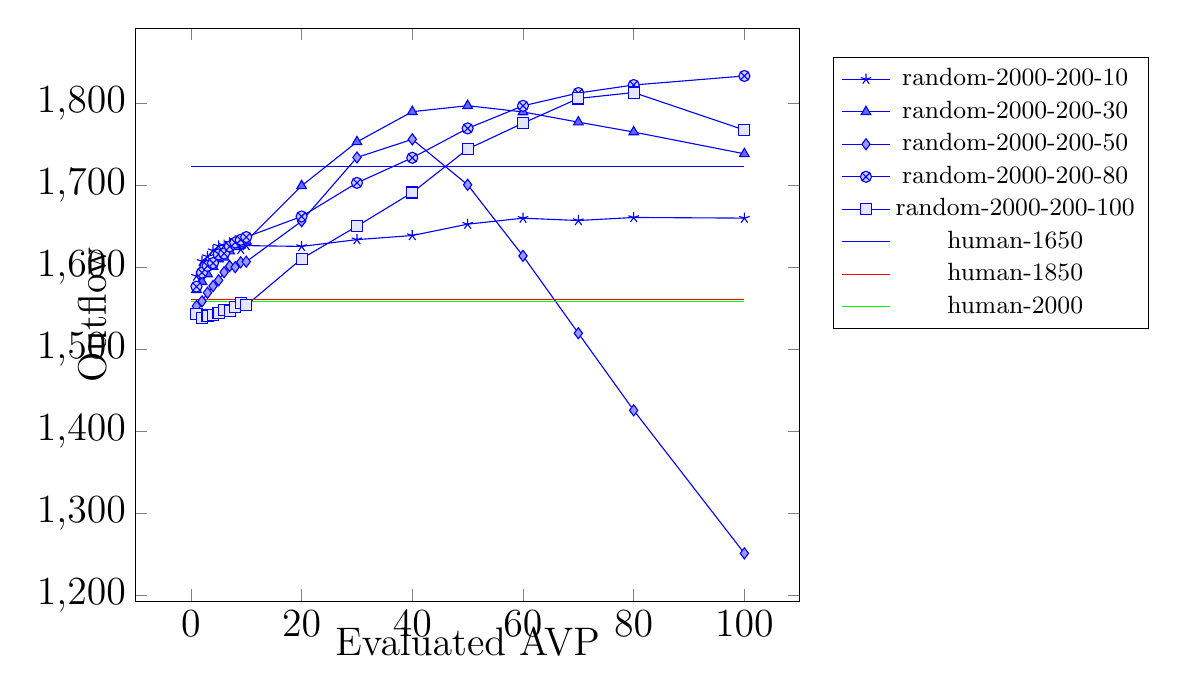
\begin{tikzpicture}[scale=1]
  \pgfplotsset{
      scale only axis,
      every x tick label/.append style={font=\Large},
      every y tick label/.append style={font=\Large},
	legend style={at={(1.05,0.95)},anchor=north west}
  }

\pgfplotscreateplotcyclelist{mycolorlist}{%
	blue,every mark/.append style={fill=blue!80}, mark=star, error bars/.cd, y dir=both, y explicit\\%
	blue,every mark/.append style={fill=blue!60}, mark=triangle*, error bars/.cd, y dir=both, y explicit\\%
	blue,every mark/.append style={fill=blue!40}, mark=diamond*, error bars/.cd, y dir=both, y explicit\\%
	blue,every mark/.append style={fill=blue!20}, mark=otimes*, error bars/.cd, y dir=both, y explicit\\%
	blue,every mark/.append style={fill=blue!10}, mark=square*, error bars/.cd, y dir=both, y explicit\\%
	red,densely dashed,every mark/.append style={solid,fill=red!80}, mark=star, error bars/.cd, y dir=both, y explicit\\%
	red,densely dashed,every mark/.append style={solid,fill=red!60},mark=triangle*, error bars/.cd, y dir=both, y explicit\\%
	red,densely dashed,every mark/.append style={solid,fill=red!40},mark=diamond*, error bars/.cd, y dir=both, y explicit\\%
	red,densely dashed,every mark/.append style={solid,fill=red!20}, mark=otimes*, error bars/.cd, y dir=both, y explicit\\%
	red,densely dashed,every mark/.append style={solid,fill=red!10}, mark=square*, error bars/.cd, y dir=both, y explicit\\%
	green!40!black, dashed,every mark/.append style={solid,fill=green!80}, mark=star, error bars/.cd, y dir=both, y explicit\\%
	green!40!black, dashed,every mark/.append style={solid,fill=green!60},mark=triangle*, error bars/.cd, y dir=both, y explicit\\%
	green!40!black, dashed,every mark/.append style={solid,fill=green!40},mark=diamond*, error bars/.cd, y dir=both, y explicit\\%
	green!40!black, dashed,every mark/.append style={solid,fill=green!20},mark=otimes*, error bars/.cd, y dir=both, y explicit\\%
	green!40!black, dashed,every mark/.append style={solid,fill=green!10},mark=square*, error bars/.cd, y dir=both, y explicit\\%
	black, dashed,every mark/.append style={solid,fill=green!80}, mark=star, error bars/.cd, y dir=both, y explicit\\%
	black, dashed,every mark/.append style={solid,fill=green!60},mark=triangle*, error bars/.cd, y dir=both, y explicit\\%
	black, dashed,every mark/.append style={solid,fill=green!40},mark=diamond*, error bars/.cd, y dir=both, y explicit\\%
	black, dashed,every mark/.append style={solid,fill=green!20},mark=otimes*, error bars/.cd, y dir=both, y explicit\\%
	black, dashed,every mark/.append style={solid,fill=green!10},mark=square*, error bars/.cd, y dir=both, y explicit\\%
	}


\begin{axis}[
    legend style={font=\small},
	ylabel={\Large Outflow},
	x label style={at={(axis description cs:0.5,-0.03)},anchor=north},
	y label style={at={(axis description cs:-0.030,0.5)}, anchor=south},
	xlabel={\Large Evaluated AVP},
	cycle list name=mycolorlist
]

\addplot table [x=a, y=b] {
a	 b	 c
1	1588.97	23.97
2	1607.11	28.43
3	1612.8	33.26
4	1620.22	31.89
5	1625.76	33.1
6	1626.59	37.51
7	1629.4	38.95
8	1632.53	38.41
9	1621.44	38.75
10	1626.19	39.85
20	1625.18	55.53
30	1633.46	62.2
40	1638.47	64.66
50	1652.33	57.81
60	1659.64	63.65
70	1656.76	60.32
80	1660.5	67.8
100	1659.71	60.72
};
\label{random-2000-200-10}

\addplot table [x=a, y=b] {
a	 b	 c
1	1572.41	19.98
2	1582.13	24.09
3	1591.6	26.05
4	1600.56	25.34
5	1609.85	29.94
6	1611.86	28.92
7	1619.42	33.57
8	1624.68	33.36
9	1628.06	35.41
10	1631.7	37.63
20	1699.06	51.78
30	1752.66	45.61
40	1789.49	40.24
50	1796.8	35.17
60	1789.16	27.63
70	1776.74	23.85
80	1764.68	22.28
100	1738.12	20.54
};
\label{random-2000-200-30}

\addplot table [x=a, y=b] {
a	 b	 c
1	1552.43	21.64
2	1558.22	23.81
3	1568.7	24.87
4	1576.91	28.45
5	1583.89	26.32
6	1593.76	24.14
7	1601.28	26.25
8	1599.91	25.88
9	1605.85	23.51
10	1606.57	25.17
20	1655.89	39.69
30	1733.69	42.81
40	1755.76	32.22
50	1700.32	28.5
60	1613.66	29.37
70	1519.31	24.89
80	1425.35	23.16
100	1250.93	13.53
};
\label{random-2000-200-50}

\addplot table [x=a, y=b] {
a	 b	 c
1	1576.15	20.83
2	1593.22	24.12
3	1601.42	24.88
4	1604.88	25.46
5	1615.43	25.05
6	1616.54	24.62
7	1625.18	28.72
8	1629.97	29.97
9	1633.28	26.43
10	1636.6	31.91
20	1661.76	37.41
30	1702.66	46.2
40	1733.29	45.85
50	1769.11	41.74
60	1796.62	50.85
70	1812.28	43.5
80	1822.03	38.52
100	1833.05	28.13
};
\label{random-2000-200-80}

\addplot table [x=a, y=b] {
a	 b	 c
1	1542.42	21.4
2	1538.17	24.73
3	1540.91	24.84
4	1541.41	24.02
5	1544.18	24.05
6	1547.89	26.39
7	1546.16	26.71
8	1551.13	25.57
9	1555.99	24.34
10	1553.33	31.63
20	1610.14	31.2
30	1649.81	37.33
40	1690.96	39.8
50	1743.91	48.43
60	1775.48	46.57
70	1805.62	43.04
80	1812.85	32.58
100	1767.13	23.87
};
\label{random-2000-200-100}

\addplot[blue, samples=200] coordinates {(0,1722.200000) (100,1722.200000)};\label{human-1650}\addplot[red, samples=200] coordinates {(0,1560.380000) (100,1560.380000)};\label{human-1850}\addplot[green, samples=200] coordinates {(0,1558.120000) (100,1558.120000)};\label{human-2000}\addlegendimage{/pgfplots/refstyle=random-2000-200-10}
\addlegendentry{random-2000-200-10}
\addlegendimage{/pgfplots/refstyle=random-2000-200-30}
\addlegendentry{random-2000-200-30}
\addlegendimage{/pgfplots/refstyle=random-2000-200-50}
\addlegendentry{random-2000-200-50}
\addlegendimage{/pgfplots/refstyle=random-2000-200-80}
\addlegendentry{random-2000-200-80}
\addlegendimage{/pgfplots/refstyle=random-2000-200-100}
\addlegendentry{random-2000-200-100}
\addlegendimage{/pgfplots/refstyle=human-1650}
\addlegendentry{human-1650}
\addlegendimage{/pgfplots/refstyle=human-1850}
\addlegendentry{human-1850}
\addlegendimage{/pgfplots/refstyle=human-2000}
\addlegendentry{human-2000}


\end{axis}
\end{tikzpicture}
\end{document}
